\documentclass[12pt]{article}%
\usepackage{amsfonts}
\usepackage{fancyhdr}
\usepackage{comment}
\usepackage{listings}
\usepackage[a4paper, top=2.5cm, bottom=2.5cm, left=2.2cm, right=2.2cm]%
{geometry}
\usepackage{times}
\usepackage{amsmath}
\usepackage{changepage}
\usepackage{amssymb}
\usepackage{graphicx}%
\setcounter{MaxMatrixCols}{30}
\newtheorem{theorem}{Theorem}
\newtheorem{acknowledgement}[theorem]{Acknowledgement}
\newtheorem{algorithm}[theorem]{Algorithm}
\newtheorem{axiom}{Axiom}
\newtheorem{case}[theorem]{Case}
\newtheorem{claim}[theorem]{Claim}
\newtheorem{conclusion}[theorem]{Conclusion}
\newtheorem{condition}[theorem]{Condition}
\newtheorem{conjecture}[theorem]{Conjecture}
\newtheorem{corollary}[theorem]{Corollary}
\newtheorem{criterion}[theorem]{Criterion}
\newtheorem{definition}[theorem]{Definition}
\newtheorem{example}[theorem]{Example}
\newtheorem{exercise}[theorem]{Exercise}
\newtheorem{lemma}[theorem]{Lemma}
\newtheorem{notation}[theorem]{Notation}
\newtheorem{problem}[theorem]{Problem}
\newtheorem{proposition}[theorem]{Proposition}
\newtheorem{remark}[theorem]{Remark}
\newtheorem{solution}[theorem]{Solution}
\newtheorem{summary}[theorem]{Summary}
\newenvironment{proof}[1][Proof]{\textbf{#1.} }{\ \rule{0.5em}{0.5em}}

\newcommand{\Q}{\mathbb{Q}}
\newcommand{\R}{\mathbb{R}}
\newcommand{\C}{\mathbb{C}}
\newcommand{\Z}{\mathbb{Z}}

\begin{document}

\title{EE460J - Lab 1}
\author{Can Gokalp, (EID: CG39283), Priyadarshan Patil (EID:PP22352)}
\date{\today}
\maketitle

\section{Programming questions}

The following libraries have been used to solve various questions: Numpy, Pandas, Matplotlib. The code snippet to import them can be found with the code for problem 1. 

\subsection{Problem 1}

Create 1000 samples from a Gaussian distribution with mean -10 and standard deviation 5. Create another 1000 samples from another independent Gaussian with mean 10 and standard deviation 5. 
\begin{enumerate}
    \item Take the sum of 2 these Gaussians by adding the two sets of 1000 points, point by point, and plot the histogram of the resulting 1000 points. What do you observe?
    \item Estimate the mean and the variance of the sum.
\end{enumerate}


\subsubsection{Solution to problem 1}

The histogram can be seen in Figure \ref{fig:hist_Q1}. It appears roughly bell shaped, centered around zero and with a wider spread than either of the base Gaussian distributions. Mathematically, the expected value of this sum should be zero and the variance be 50. Due to sampling, the expected value is 0.0088 and the variance is 51.07.\\

\begin{figure}[h]
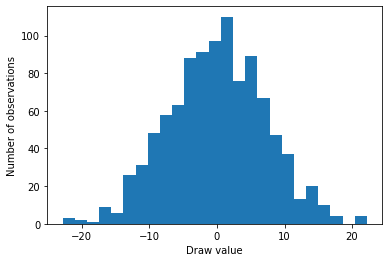
\includegraphics[scale=0.6]{Plots/hist_Q1.png}
\centering
\caption{Histogram of addition of 1000 draws from two Gaussian distributions}
\label{fig:hist_Q1}
\centering
\end{figure}

\subsubsection{Code for problem 1}
\begin{lstlisting}
import pandas as pd
import matplotlib.pyplot as plt
import numpy as np

mu1 = -10
sigma1 = 5
obs1 = np.random.normal(mu1, sigma1, 1000)

mu2 = 10
sigma2 = 5
obs2 = np.random.normal(mu2, sigma2, 1000)

obs3 = np.add(obs1, obs2)
labels = ['Value', 'Number of observations']
plt.hist(obs3,bins=25,label=labels)
plt.xlabel('Draw value')
plt.ylabel('Number of observations')

obs3_mu = np.mean(obs3)

obs3_sigma = np.std(obs3)

print("The mean of the sum of the two 1000 point draws is: ",obs3_mu,"
and the standard deviation is: ",obs3_sigma)
\end{lstlisting}

%-------------------------------------------------------

\subsection{Problem 2}

Let $X_i$ be an i.i.d. Bernoulli random variable with value {-1,1}. Look at the random variable $Z_n = (\frac{1}{\sqrt{n}})\Sigma X_i$. By taking 1000 draws from $Z_n$, plot its histogram. Check that for small $n$ (say, 5-10) $Z_n$ does not look that much like a Gaussian, but when $n$ is bigger (already by the time $n$ = 30 or 50) it looks much more like a Gaussian. Check also for much bigger $n$: $n$ = 250, to see that at this point, one can really see the bell curve.\\


\subsubsection{Solution to problem 2}

The histograms can be seen in Figure \ref{fig:hist_Q2}. For $n=5$, we see six unique values and a vaguely Gaussian pattern, but that is not verified mathematically. For $n=30$, the distribution Gaussian, but skewed to the left. For $n=50$, the histogram appears bi-modal. For n=250, the histogram is much closer to a bell curve with neat separations into bins. \\

\begin{figure}[h]
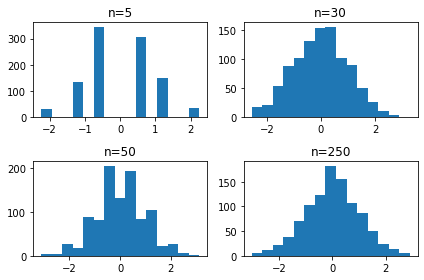
\includegraphics[scale=0.8]{Plots/figs_Q2.png}
\centering
\caption{Histogram of 1000 $Z_n$ draws for $n \in {5, 30, 50, 250}$}
\label{fig:hist_Q2}
\centering
\end{figure}

\subsubsection{Code for problem 2}
\begin{lstlisting}
def draw_Z(num_draws):
    temp_array = np.random.binomial(size=num_draws, n=1, p= 0.5)
    temp_array[temp_array == 0] = -1
    Z = (np.sum(temp_array)/np.sqrt(num_draws))
    return (Z)

figure, axes = plt.subplots(nrows=2, ncols=2)

num_draws=5
int_array = np.zeros(1000)
for i in range(1000):
    int_array[i] = draw_Z(num_draws)
#print(int_array)
axes[0,0].hist(int_array, bins = 15)
axes[0, 0].set_title('n=5')

num_draws=30
int_array = np.zeros(1000)
for i in range(1000):
    int_array[i] = draw_Z(num_draws)
#print(int_array)
axes[0,1].hist(int_array, bins = 15)
axes[0,1].set_title('n=30')

num_draws=50
int_array = np.zeros(1000)
for i in range(1000):
    int_array[i] = draw_Z(num_draws)
#print(int_array)
axes[1,0].hist(int_array, bins = 15)
axes[1,0].set_title('n=50')

num_draws=250
int_array = np.zeros(1000)
for i in range(1000):
    int_array[i] = draw_Z(num_draws)
#print(int_array)
axes[1,1].hist(int_array, bins = 15)
axes[1,1].set_title('n=250')

figure.tight_layout()
\end{lstlisting}

%-------------------------------------------------------

\subsection{Problem 3}

Estimate the mean and standard deviation from 1 dimensional data: generate 25,000 samples from a Gaussian distribution with mean 0 and standard deviation 5. Then estimate the mean and standard deviation of this gaussian using elementary numpy commands, i.e., addition, multiplication, division (do not use a command that takes data and returns the mean or standard deviation).\\

\subsubsection{Solution to problem 3}

The numpy library was used to generate 25,000 samples from a \textit{\textbf{N}}(0, 5) Gaussian distribution. The mean was calculated by summing all values and dividing the resulting sum by the number of observations. The standard deviation was obtained by the definition of variance, i.e, $Var[X] = \frac{\Sigma_i (x_i-E[X])^2}{n-1}$, and $StDev. = \sqrt{Var}$. For this sample, the mean was 0.036 and the standard deviation was 5.009.\\

\subsubsection{Code for problem 3}
\begin{lstlisting}
mu4 = 0
sigma4 = 5
num_obs4 = 25000
obs4 = np.random.normal(mu4, sigma4, num_obs4)

mean_obs4 = np.sum(obs4)/num_obs4
int_array1 = np.full((num_obs4), mean_obs4)
int_array2 = np.subtract(obs4,int_array1)
int_array3 = np.multiply(int_array2,int_array2)
stdev_obs4 = np.sqrt(np.sum(int_array3)/(num_obs4-1))

print("The calculated mean is: ",mean_obs4,"
and the standard deviation is: ",stdev_obs4)
\end{lstlisting}


%-------------------------------------------------------

\subsection{Problem 4}

Estimate the mean and covariance matrix for multi-dimensional data: generate 10,000 samples of 2 dimensional data from the Gaussian distribution. 

\begin{align*}
\begin{pmatrix}X_{i}\\
Y_{i}
\end{pmatrix} &\sim  N
\begin{pmatrix}
\begin{pmatrix}
-5\\
5
\end{pmatrix}\ ,&
\begin{pmatrix}
20 & 0.8\\
0.8 & 30
\end{pmatrix}
\end{pmatrix}\\
\end{align*}

Then, estimate the mean and covariance matrix for this multi-dimensional data using elementary numpy commands, i.e., addition, multiplication, division (do not use a command that takes data and returns the mean or standard deviation).\\

\subsubsection{Solution to problem 4}

The workflow for calculation of the mean was similar to the previous problem. The draws for a variable were summed and averaged across the number of observations. For the covariance matrix, the vector formula taught in class was used. First, the $D_{cent}$ matrix was calculated by subtracting the mean value from each draw. Then, the matrix is calculated as:

\begin{equation}
    Covariance\ matrix = \frac{1}{n-1}(D_{cent}^T)D_{cent}
\end{equation}

\noindent It is observed that the mean array is $\begin{pmatrix}-5.005\\5.118\end{pmatrix}$ and the covariance matrix is $\begin{pmatrix}19.464 & 0.833\\0.833 & 29.020\end{pmatrix}$.


\subsubsection{Code for problem 4}
\begin{lstlisting}
mean_arr = [-5, 5]
cov_mat = [[20, 0.8], [0.8, 30]]
num_obs5 = 10000

obs5 = np.empty(shape=(num_obs5,2))
for i in range(num_obs5):
    obs5[i] = np.random.multivariate_normal(mean_arr,cov_mat)

mean_arr_est = obs5.sum(axis=0)/num_obs5
print(mean_arr_est)

int_array4 = np.full([num_obs5,2], mean_arr_est)
D_cent = np.subtract(obs5,int_array4)
temp_array = np.matmul(np.transpose(D_cent),D_cent)
print(temp_array/(num_obs5-1))\\
\end{lstlisting}

%-------------------------------------------------------

\subsection{Problem 5}

Download from Canvas/Files the dataset \emph{PatientData.csv}. Each row is a patient and the last column is the condition that the patient has. Do data exploration using Pandas and other visualization tools to understand what you can about the dataset. For example:
\begin{enumerate}
    \item How many patients and how many features are there?
    \item What is the meaning of the first 4 features? See if you can understand what they mean.
    \item Are there missing values? Replace them with the average of the corresponding feature column
    \item How could you test which features strongly influence the patient condition and which do not? 
\end{enumerate}

List what you think are the three most important features.

\subsubsection{Solution to problem 5}

\begin{enumerate}
    \item The number of patients is 452 and the number of features is 280.
    \item The first 4 features appear to be age (years), gender/sex, height (cm), and weight (kg).
    \item There are missing values in the dataset: True. The missing values have been filled with the average of the corresponding columns.
    \item There are multiple ways for feature selection. One is using the Pearson correlation matrix, which provides the linear correlation between all features (in sets of 2). There are other methods such as recursive feature elimination and univariate feature selection, but we shall use the Pearson correlation matrix for this assignment.
\end{enumerate} 

From the Pearson correlation matrix, I think that features in column numbers 5, 91 and 93 are the three most important features.

\subsubsection{Code for problem 5}
\begin{lstlisting}
dataset = pd.read_csv("PatientData.csv", header=None)

print(dataset.head())

num_patients = dataset.shape[0]
num_features = dataset.shape[1]

#print(dataset[279].describe(percentiles = [0.05,0.25,0.5,0.75,0.95]))

print("a) The number of patients is: ",num_patients,"
and the number of features is: ",num_features)

print("b) The first 4 features appear to be age, gender,
height, and weight.")

cols = list(dataset.columns) 
dataset[cols] = pd.to_numeric(dataset[cols].stack(),
errors='coerce').unstack()

print("c) There are missing values in the dataset: ",
dataset.isnull().any().any())

dataset_1=dataset.fillna(dataset.mean())
print("The missing values have been filled with the average
of the corresponding columns.")

Pearson_mat = dataset.corr()
cor_target = abs(Pearson_mat[279])
relevant_features = cor_target[cor_target>0.3]
print(relevant_features)
\end{lstlisting}


\section{Written questions}

\subsection{Problem 1}

Consider two random variables X,Y that are not independent. Their probabilities of are given by the following table:

\begin{table}[!h]
\centering
\begin{tabular}{|l|l|l|}
\hline
    & X=0 & X=1 \\ \hline
Y=0 & 1/4 & 1/4 \\ \hline
Y=1 & 1/6 & 1/3 \\ \hline
\end{tabular}
\end{table}

\begin{enumerate}
    \item What is the probability that X = 1?
    \item What is the probability that X = 1 conditioned on Y = 1?
    \item What is the variance of the random variable X?
    \item What is the variance of the random variable X conditioned that Y = 1?
    \item What is $E[X^3 + X^2 + 3Y^7|Y = 1]$? 
\end{enumerate}

\subsubsection{Solution to problem 1}

\begin{enumerate}
    \item $P(X=1) =  1/4 + 1/3 = 7/12$
    \item $P(X=1|Y=1) = \frac{1/3}{(1/6 + 1/3)} = \frac{2}{3}$
    \item The marginal distribution of X is as follows:\\
            $P(X)= 
            \begin{cases}
            \ 5/12 ,&  X = 0\\
            \ 7/12,              & X = 1
            \end{cases}$
            \newline
            Therefore, $E[X] = 5/12 * 0 + 7/12 * 1 = 7/12$\\
            Also, $E[X^2] = 5/12 * 0 + 7/12 * 1 = 7/12$\\
            Therefore, Var[X] = $E[X^2] - E[X]^2 = 7/12 - 49/144 = \frac{35}{144}$
            
    \item The marginal distribution of X is as follows:\\
            $P(X|Y=1)= 
            \begin{cases}
            \ 1/3 ,&  X = 0\\
            \ 2/3 ,& X = 1
            \end{cases}$
            \newline
            Therefore, $E[X|Y=1] = 1/3 * 0 + 2/3 * 1 = 2/3$\\
            Also, $E[X^2|Y=1] = 1/3 * 0 + 2/3 * 1 = 2/3$\\
            Therefore, Var[X|Y=1] = $E[X^2] - E[X]^2 = 2/3 - 4/9 = \frac{2}{9}$
    \item The same marginal distribution from the previous part is valid here. Therefore\\
    $E[X^3 + X^2 + 3Y^7|Y = 1] = E[X^3|Y=1] + E[X^2|Y=1] + 3E[Y^7|Y=1]$\\
    $E[X^3 + X^2 + 3Y^7|Y = 1] = 2/3 + 2/3 + 3*1 = 4\frac{1}{3} = \frac{13}{3}$
\end{enumerate}

%-------------------------------------------------------

\subsection{Problem 2}

Consider the vectors $v_1 = [1, 1, 1]$ and $v_2 = [1, 0, 0]$. These two vectors define a 2-dimensional subspace of $\mathbf{R}^3$. Project the points $P_1 = [3, 3, 3], P_2 = [1, 2, 3], P_3 = [0, 0, 1]$ on this subspace. Write down the coordinates of the three projected points. (You can use numpy or a calculator to do arithmetic if you want).

\subsubsection{Solution to problem 2}
The dot product of $v_1$ and $v_2$ is not zero. Also, $v_1$ is not a unit vector, so it is now written as $[1/3, 1/3, 1/3]$ Therefore, we need to find an orthogonal basis. That is done by projecting $v_1$ onto $v_2$. So, $v_1^\perp = v_1 - proj_{v_2}v_1 = v_1 - \frac{v_1^T v_2}{v_2^T v_2}v_2 = [0, 1/3, 1/3]$.\\ 

Normalizing them, we have the basis vectors as $[0, 1/2, 1/2]$ and $[1, 0, 0]$. Now, we have a perpendicular set of vectors $v_1^\perp$ and $v_2$, defining the subspace. Projecting the three points on the subspace is a standard orthogonal projection. The formula is given below:\\
$P^\perp$ = $Proj_{v_1^\perp} P + Proj_{v_2} P = \frac{P^\perp v_1^\perp}{(v_1^\perp)^T v_1^\perp} v_1^\perp + \frac{P^\perp v_2}{(v_2)^T v_2} v_2 \qquad \forall P \in \{P_1, P_2, P_3\}$\\

Therefore, the projections of $P_1, P_2, and P_3$ on the subspace are: $[2/3, 2/3, 2/3]$, $[1/4, 1/2, 3/4]$, and $[0, 0, 1/2]$, respectively.

%-------------------------------------------------------

\subsection{Problem 3}

Consider a coin such that probability of heads is 2/3. Suppose you toss the coin 100 times. Estimate the probability of getting 50 or fewer heads. You can do this in a variety of ways. One way is to use the Central Limit Theorem. Be explicit in your calculations and tell us what tools you are using in these.

\subsubsection{Solution to problem 3}

We use the Normal approximation for the Binomial distribution with large number of experiments. This is using Central Limit Theorem to identify the sum of 100 Binomial trials as a normal distribution. If $X \sim B(n, p)$ and if $n$ is large and/or p is close to 1/2, then X is approximately $N(np, np(1-p))$. Therefore, the given scenario, the number of heads can be approximated by $H \sim N(66.67, 22.23)$. Then, it is trivial to calculate $P(H<50.5)$. Note that H is less than 50.5 to account for the continuity assumption. The tool used for CDF calculation is a standard normal table.\\

\noindent $P(H<50.5) = 23.35\%$.

%-------------------------------------------------------

\end{document}
